% Options for packages loaded elsewhere
\PassOptionsToPackage{unicode}{hyperref}
\PassOptionsToPackage{hyphens}{url}
\PassOptionsToPackage{dvipsnames,svgnames,x11names}{xcolor}
%
\documentclass[
  letterpaper,
  DIV=11,
  numbers=noendperiod]{scrreprt}

\usepackage{amsmath,amssymb}
\usepackage{iftex}
\ifPDFTeX
  \usepackage[T1]{fontenc}
  \usepackage[utf8]{inputenc}
  \usepackage{textcomp} % provide euro and other symbols
\else % if luatex or xetex
  \usepackage{unicode-math}
  \defaultfontfeatures{Scale=MatchLowercase}
  \defaultfontfeatures[\rmfamily]{Ligatures=TeX,Scale=1}
\fi
\usepackage{lmodern}
\ifPDFTeX\else  
    % xetex/luatex font selection
\fi
% Use upquote if available, for straight quotes in verbatim environments
\IfFileExists{upquote.sty}{\usepackage{upquote}}{}
\IfFileExists{microtype.sty}{% use microtype if available
  \usepackage[]{microtype}
  \UseMicrotypeSet[protrusion]{basicmath} % disable protrusion for tt fonts
}{}
\makeatletter
\@ifundefined{KOMAClassName}{% if non-KOMA class
  \IfFileExists{parskip.sty}{%
    \usepackage{parskip}
  }{% else
    \setlength{\parindent}{0pt}
    \setlength{\parskip}{6pt plus 2pt minus 1pt}}
}{% if KOMA class
  \KOMAoptions{parskip=half}}
\makeatother
\usepackage{xcolor}
\setlength{\emergencystretch}{3em} % prevent overfull lines
\setcounter{secnumdepth}{5}
% Make \paragraph and \subparagraph free-standing
\makeatletter
\ifx\paragraph\undefined\else
  \let\oldparagraph\paragraph
  \renewcommand{\paragraph}{
    \@ifstar
      \xxxParagraphStar
      \xxxParagraphNoStar
  }
  \newcommand{\xxxParagraphStar}[1]{\oldparagraph*{#1}\mbox{}}
  \newcommand{\xxxParagraphNoStar}[1]{\oldparagraph{#1}\mbox{}}
\fi
\ifx\subparagraph\undefined\else
  \let\oldsubparagraph\subparagraph
  \renewcommand{\subparagraph}{
    \@ifstar
      \xxxSubParagraphStar
      \xxxSubParagraphNoStar
  }
  \newcommand{\xxxSubParagraphStar}[1]{\oldsubparagraph*{#1}\mbox{}}
  \newcommand{\xxxSubParagraphNoStar}[1]{\oldsubparagraph{#1}\mbox{}}
\fi
\makeatother


\providecommand{\tightlist}{%
  \setlength{\itemsep}{0pt}\setlength{\parskip}{0pt}}\usepackage{longtable,booktabs,array}
\usepackage{calc} % for calculating minipage widths
% Correct order of tables after \paragraph or \subparagraph
\usepackage{etoolbox}
\makeatletter
\patchcmd\longtable{\par}{\if@noskipsec\mbox{}\fi\par}{}{}
\makeatother
% Allow footnotes in longtable head/foot
\IfFileExists{footnotehyper.sty}{\usepackage{footnotehyper}}{\usepackage{footnote}}
\makesavenoteenv{longtable}
\usepackage{graphicx}
\makeatletter
\newsavebox\pandoc@box
\newcommand*\pandocbounded[1]{% scales image to fit in text height/width
  \sbox\pandoc@box{#1}%
  \Gscale@div\@tempa{\textheight}{\dimexpr\ht\pandoc@box+\dp\pandoc@box\relax}%
  \Gscale@div\@tempb{\linewidth}{\wd\pandoc@box}%
  \ifdim\@tempb\p@<\@tempa\p@\let\@tempa\@tempb\fi% select the smaller of both
  \ifdim\@tempa\p@<\p@\scalebox{\@tempa}{\usebox\pandoc@box}%
  \else\usebox{\pandoc@box}%
  \fi%
}
% Set default figure placement to htbp
\def\fps@figure{htbp}
\makeatother
% definitions for citeproc citations
\NewDocumentCommand\citeproctext{}{}
\NewDocumentCommand\citeproc{mm}{%
  \begingroup\def\citeproctext{#2}\cite{#1}\endgroup}
\makeatletter
 % allow citations to break across lines
 \let\@cite@ofmt\@firstofone
 % avoid brackets around text for \cite:
 \def\@biblabel#1{}
 \def\@cite#1#2{{#1\if@tempswa , #2\fi}}
\makeatother
\newlength{\cslhangindent}
\setlength{\cslhangindent}{1.5em}
\newlength{\csllabelwidth}
\setlength{\csllabelwidth}{3em}
\newenvironment{CSLReferences}[2] % #1 hanging-indent, #2 entry-spacing
 {\begin{list}{}{%
  \setlength{\itemindent}{0pt}
  \setlength{\leftmargin}{0pt}
  \setlength{\parsep}{0pt}
  % turn on hanging indent if param 1 is 1
  \ifodd #1
   \setlength{\leftmargin}{\cslhangindent}
   \setlength{\itemindent}{-1\cslhangindent}
  \fi
  % set entry spacing
  \setlength{\itemsep}{#2\baselineskip}}}
 {\end{list}}
\usepackage{calc}
\newcommand{\CSLBlock}[1]{\hfill\break\parbox[t]{\linewidth}{\strut\ignorespaces#1\strut}}
\newcommand{\CSLLeftMargin}[1]{\parbox[t]{\csllabelwidth}{\strut#1\strut}}
\newcommand{\CSLRightInline}[1]{\parbox[t]{\linewidth - \csllabelwidth}{\strut#1\strut}}
\newcommand{\CSLIndent}[1]{\hspace{\cslhangindent}#1}

\KOMAoption{captions}{tableheading}
\makeatletter
\@ifpackageloaded{tcolorbox}{}{\usepackage[skins,breakable]{tcolorbox}}
\@ifpackageloaded{fontawesome5}{}{\usepackage{fontawesome5}}
\definecolor{quarto-callout-color}{HTML}{909090}
\definecolor{quarto-callout-note-color}{HTML}{0758E5}
\definecolor{quarto-callout-important-color}{HTML}{CC1914}
\definecolor{quarto-callout-warning-color}{HTML}{EB9113}
\definecolor{quarto-callout-tip-color}{HTML}{00A047}
\definecolor{quarto-callout-caution-color}{HTML}{FC5300}
\definecolor{quarto-callout-color-frame}{HTML}{acacac}
\definecolor{quarto-callout-note-color-frame}{HTML}{4582ec}
\definecolor{quarto-callout-important-color-frame}{HTML}{d9534f}
\definecolor{quarto-callout-warning-color-frame}{HTML}{f0ad4e}
\definecolor{quarto-callout-tip-color-frame}{HTML}{02b875}
\definecolor{quarto-callout-caution-color-frame}{HTML}{fd7e14}
\makeatother
\makeatletter
\@ifpackageloaded{bookmark}{}{\usepackage{bookmark}}
\makeatother
\makeatletter
\@ifpackageloaded{caption}{}{\usepackage{caption}}
\AtBeginDocument{%
\ifdefined\contentsname
  \renewcommand*\contentsname{Table of contents}
\else
  \newcommand\contentsname{Table of contents}
\fi
\ifdefined\listfigurename
  \renewcommand*\listfigurename{List of Figures}
\else
  \newcommand\listfigurename{List of Figures}
\fi
\ifdefined\listtablename
  \renewcommand*\listtablename{List of Tables}
\else
  \newcommand\listtablename{List of Tables}
\fi
\ifdefined\figurename
  \renewcommand*\figurename{Figure}
\else
  \newcommand\figurename{Figure}
\fi
\ifdefined\tablename
  \renewcommand*\tablename{Table}
\else
  \newcommand\tablename{Table}
\fi
}
\@ifpackageloaded{float}{}{\usepackage{float}}
\floatstyle{ruled}
\@ifundefined{c@chapter}{\newfloat{codelisting}{h}{lop}}{\newfloat{codelisting}{h}{lop}[chapter]}
\floatname{codelisting}{Listing}
\newcommand*\listoflistings{\listof{codelisting}{List of Listings}}
\makeatother
\makeatletter
\makeatother
\makeatletter
\@ifpackageloaded{caption}{}{\usepackage{caption}}
\@ifpackageloaded{subcaption}{}{\usepackage{subcaption}}
\makeatother

\usepackage{bookmark}

\IfFileExists{xurl.sty}{\usepackage{xurl}}{} % add URL line breaks if available
\urlstyle{same} % disable monospaced font for URLs
\hypersetup{
  pdftitle={ELSTE Data Science Master Course},
  pdfauthor={Sébastien Biass \& Stéphane Guerrier},
  colorlinks=true,
  linkcolor={blue},
  filecolor={Maroon},
  citecolor={Blue},
  urlcolor={Blue},
  pdfcreator={LaTeX via pandoc}}


\title{ELSTE Data Science Master Course}
\usepackage{etoolbox}
\makeatletter
\providecommand{\subtitle}[1]{% add subtitle to \maketitle
  \apptocmd{\@title}{\par {\large #1 \par}}{}{}
}
\makeatother
\subtitle{A rapid introduction to data science using Python}
\author{Sébastien Biass \& Stéphane Guerrier}
\date{2025-01-01}

\begin{document}
\maketitle

\renewcommand*\contentsname{Table of contents}
{
\hypersetup{linkcolor=}
\setcounter{tocdepth}{2}
\tableofcontents
}

\bookmarksetup{startatroot}

\chapter*{Preface}\label{preface}
\addcontentsline{toc}{chapter}{Preface}

\markboth{Preface}{Preface}

This is a Quarto book.

To learn more about Quarto books visit
\url{https://quarto.org/docs/books}.

\part{Class 1}

\chapter*{Class 1}\label{class-1-1}
\addcontentsline{toc}{chapter}{Class 1}

\markboth{Class 1}{Class 1}

\section*{Today's objectives}\label{todays-objectives}
\addcontentsline{toc}{section}{Today's objectives}

\markright{Today's objectives}

\subsection*{Theory}\label{theory}
\addcontentsline{toc}{subsection}{Theory}

\begin{enumerate}
\def\labelenumi{\arabic{enumi}.}
\tightlist
\item
  Why scientific coding?
\item
  Fundamentals of scientific computing
\item
  Why Python?
\item
  How to use Python?
\end{enumerate}

\chapter{Summary}\label{summary}

In summary, this book has no content whatsoever.

\part{Appendices}

\chapter*{Setup VS Code}\label{setup-vs-code}
\addcontentsline{toc}{chapter}{Setup VS Code}

\markboth{Setup VS Code}{Setup VS Code}

This tutorial guides you through the installation and configuration of
Visual Studio Code (VS Code) for Python development in the 0013 computer
room at the University of Geneva.

\section*{Open VS Code}\label{open-vs-code}
\addcontentsline{toc}{section}{Open VS Code}

\markright{Open VS Code}

\begin{enumerate}
\def\labelenumi{\arabic{enumi}.}
\tightlist
\item
  Create a folder on your \texttt{H:/} drive named
  \texttt{data\_science}
\item
  Open \texttt{VS\ Code}
\item
  Click \texttt{File\ /\ Open\ Folder} and choose the
  \texttt{data\_science} folder (Figure~\ref{fig-open})
\item
  When asked, click to confirm your trust in the system
\end{enumerate}

These steps will ensure that Python works and finds the files in this
exact folder.

\begin{figure}

\centering{

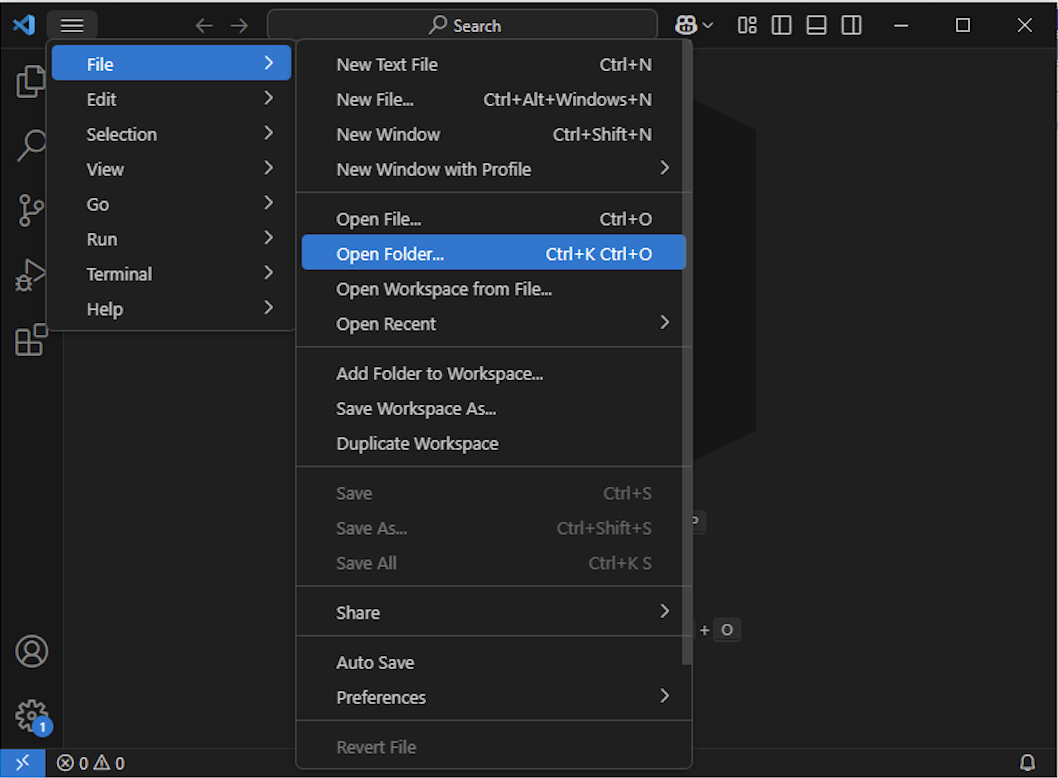
\includegraphics[width=0.8\linewidth,height=\textheight,keepaspectratio]{appendices/img/1.png}

}

\caption{\label{fig-open}Open VS Code and set the working folder}

\end{figure}%

\section*{Create a new Jupyter
Notebook}\label{create-a-new-jupyter-notebook}
\addcontentsline{toc}{section}{Create a new Jupyter Notebook}

\markright{Create a new Jupyter Notebook}

\begin{enumerate}
\def\labelenumi{\arabic{enumi}.}
\tightlist
\item
  Type Ctrl + Shift + i (or Cmd + Shift + i on MacOS) to open the
  command palette
\item
  Type \texttt{jupyter} and select
  \texttt{Create:\ New\ Jupyter\ Notebook}
  (Figure~\ref{fig-newnotebook})
\end{enumerate}

\begin{figure}

\centering{

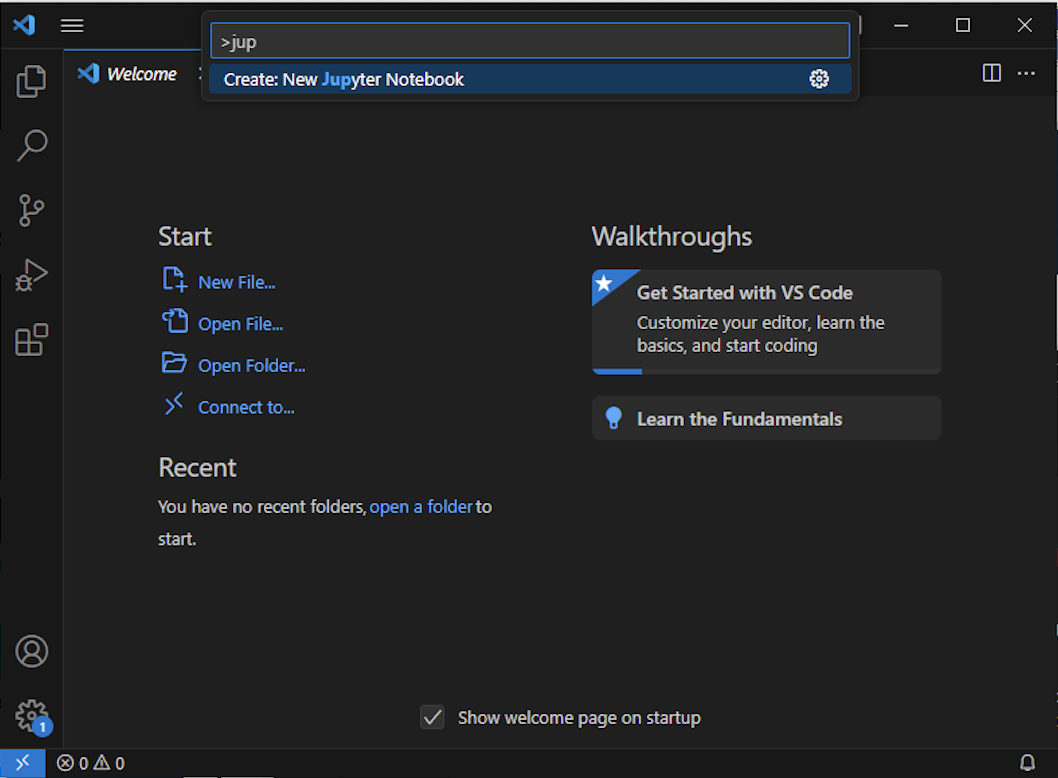
\includegraphics[width=0.8\linewidth,height=\textheight,keepaspectratio]{appendices/img/3.png}

}

\caption{\label{fig-newnotebook}Create a new Jupyter Notebook}

\end{figure}%

\begin{tcolorbox}[enhanced jigsaw, rightrule=.15mm, toprule=.15mm, coltitle=black, title=\textcolor{quarto-callout-tip-color}{\faLightbulb}\hspace{0.5em}{Command palette}, colframe=quarto-callout-tip-color-frame, bottomtitle=1mm, colback=white, breakable, titlerule=0mm, opacityback=0, opacitybacktitle=0.6, leftrule=.75mm, arc=.35mm, colbacktitle=quarto-callout-tip-color!10!white, left=2mm, toptitle=1mm, bottomrule=.15mm]

The command palette is a key functionality of VS Code, learning to use
it will speed up your workflow.

\end{tcolorbox}

\section*{Install the Python
extensions}\label{install-the-python-extensions}
\addcontentsline{toc}{section}{Install the Python extensions}

\markright{Install the Python extensions}

This step installs the Python extensions for VS Code.

\begin{enumerate}
\def\labelenumi{\arabic{enumi}.}
\tightlist
\item
  When asked, click the \texttt{Install} button and wait for it to
  finish (Figure~\ref{fig-3})
\end{enumerate}

\begin{figure}

\centering{

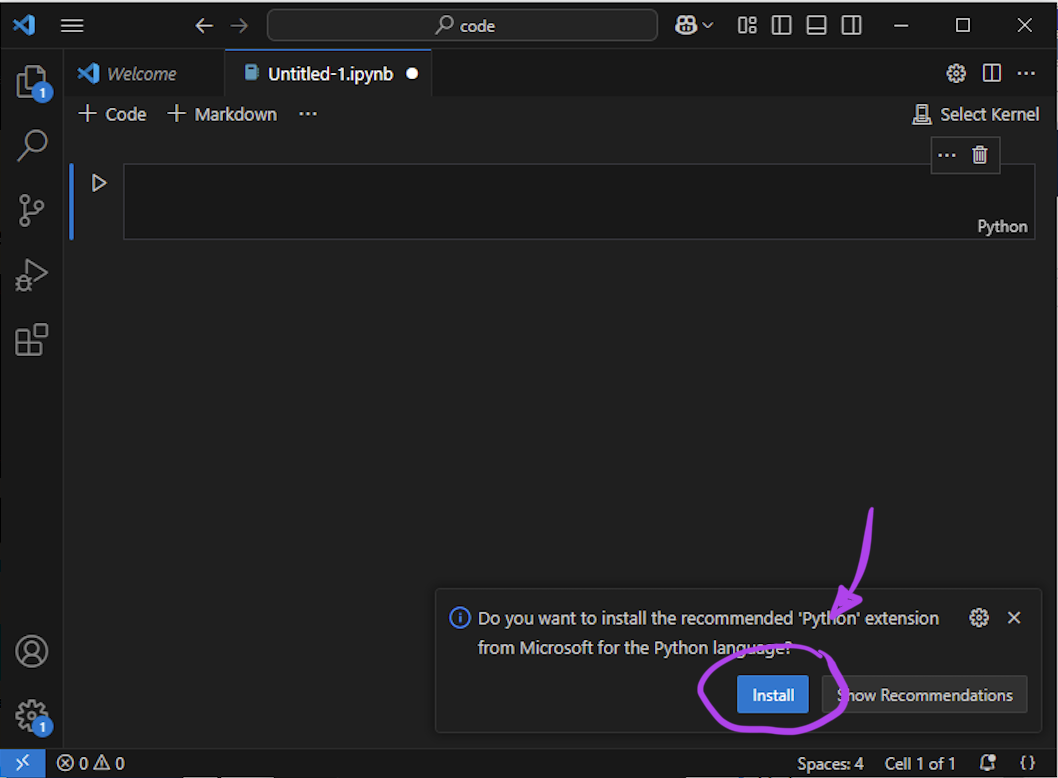
\includegraphics[width=0.8\linewidth,height=\textheight,keepaspectratio]{appendices/img/4.png}

}

\caption{\label{fig-3}Create a new Jupyter Notebook}

\end{figure}%

\section*{Install Jupyter}\label{install-jupyter}
\addcontentsline{toc}{section}{Install Jupyter}

\markright{Install Jupyter}

Jupyter Notebooks are one of the ways to run Python. This step installs
all the required Jupyter stuff for VS Code.

\begin{enumerate}
\def\labelenumi{\arabic{enumi}.}
\tightlist
\item
  On the top right corner of the notebook, locate and click on the
  \texttt{Select\ kernel} button Figure~\ref{fig-4}
\item
  Install the \texttt{Jupyter\ notebook\ support} extension
  (Figure~\ref{fig-5})
\end{enumerate}

\begin{figure}

\centering{

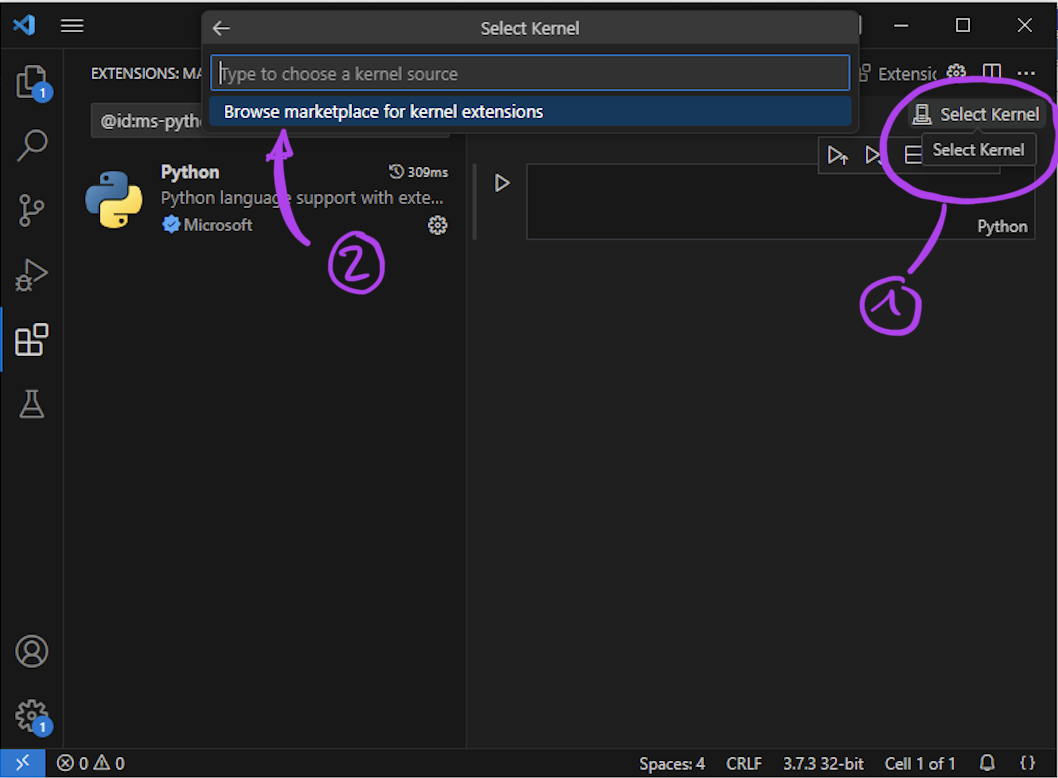
\includegraphics[width=0.8\linewidth,height=\textheight,keepaspectratio]{appendices/img/6.png}

}

\caption{\label{fig-4}Browse for kernels}

\end{figure}%

\begin{figure}

\centering{

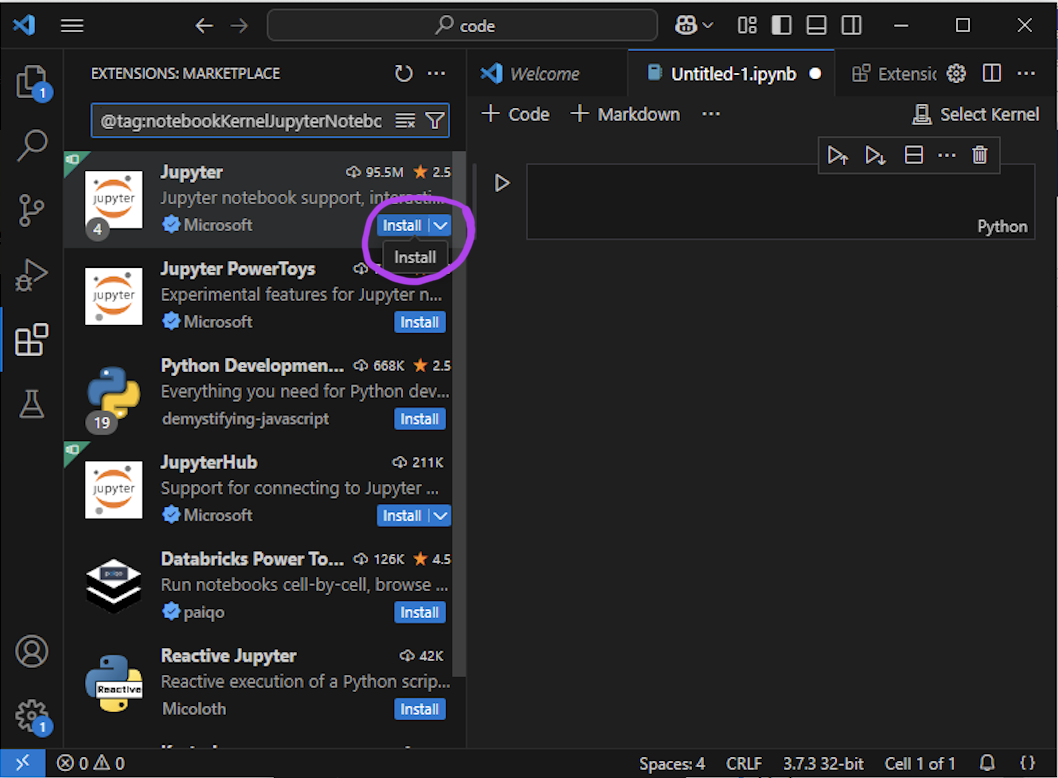
\includegraphics[width=0.8\linewidth,height=\textheight,keepaspectratio]{appendices/img/7.png}

}

\caption{\label{fig-5}Install the Jupyter notebook support extension}

\end{figure}%

\section*{Select the right Python}\label{select-the-right-python}
\addcontentsline{toc}{section}{Select the right Python}

\markright{Select the right Python}

Several versions of Python can be installed on a computer. In the
computer room, these versions are controlled by an \emph{environment
manager} called \texttt{anaconda}. This step ensures that the Jupyter
notebook will use the right Python version, i.e., the one installed
using \texttt{anaconda}.

\begin{enumerate}
\def\labelenumi{\arabic{enumi}.}
\tightlist
\item
  On the top right corner of the notebook, where the
  \texttt{Select\ kernel} button previously appeared, make sure you see
  \texttt{base\ (Python\ 3.x.x)} (Figure~\ref{fig-env})
\item
  If you don't, click on the button and search for the right one (i.e.,
  there should be \texttt{anaconda} in the path)
\end{enumerate}

\begin{figure}

\centering{

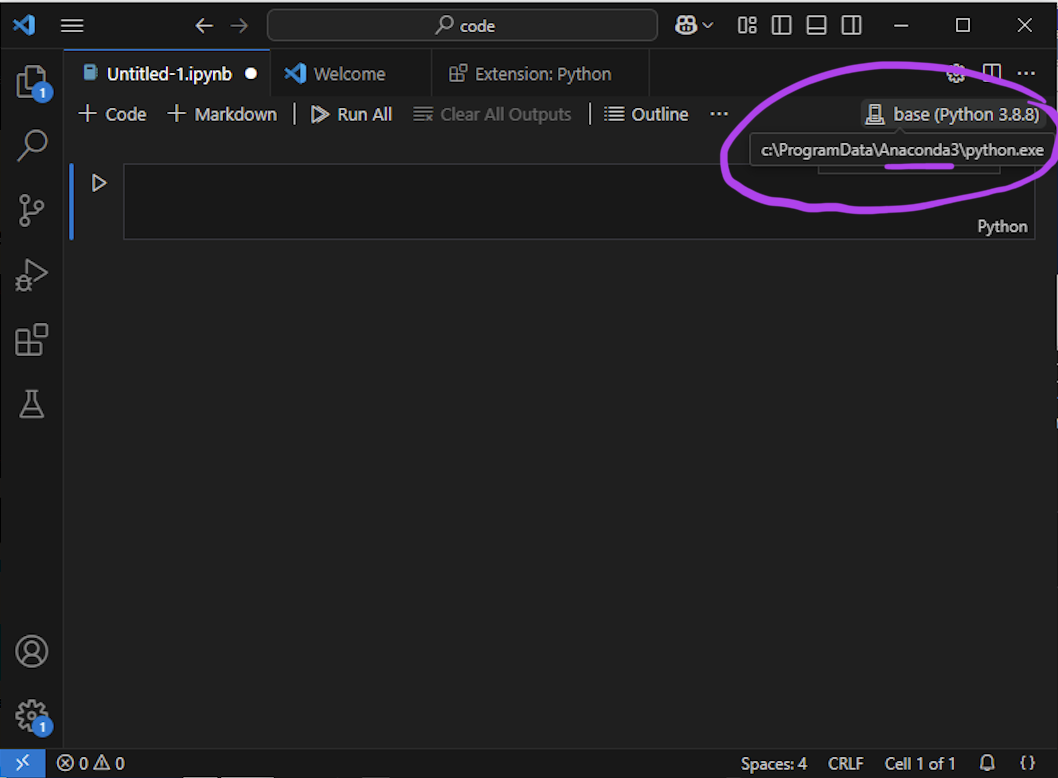
\includegraphics[width=0.8\linewidth,height=\textheight,keepaspectratio]{appendices/img/8.png}

}

\caption{\label{fig-env}Select the right Python environment}

\end{figure}%

\bookmarksetup{startatroot}

\chapter*{References}\label{references}
\addcontentsline{toc}{chapter}{References}

\markboth{References}{References}

\phantomsection\label{refs}
\begin{CSLReferences}{0}{1}
\end{CSLReferences}




\end{document}
